\chapter{SQL JOIN - Combinazione Tabelle}

\section*{Introduzione}
Il JOIN è il meccanismo SQL per combinare dati da più tabelle correlate tramite chiavi esterne. Questo capitolo presenta i diversi tipi di JOIN (INNER, LEFT, RIGHT, FULL OUTER) con diagrammi visivi e esempi pratici per comprendere come e quando usarli.

\section*{Obiettivi di apprendimento}
\begin{itemize}
    \item Comprendere il concetto di JOIN e la necessità di combinare tabelle
    \item Scrivere query con INNER JOIN
    \item Scrivere query con LEFT JOIN e RIGHT JOIN
    \item Scrivere query con FULL OUTER JOIN
    \item Usare CROSS JOIN
    \item Usare alias per tabelle nei JOIN
    \item Eseguire JOIN su più di due tabelle
    \item Evitare cartesiani (combinazioni errate)
\end{itemize}

\section{Concetti di Base}

\subsection{Perché JOIN?}
Nel modello relazionale, i dati sono distribuiti su più tabelle. Per rispondere a domande che coinvolgono dati di più tabelle, devi combinarle con JOIN.

\begin{tcolorbox}[colback=blue!10, colframe=blue!60, title=Esempio: Domanda che richiede JOIN]
``Quali clienti hanno fatto ordini nel 2023?''

Per rispondere devo:
\begin{enumerate}
    \item Trovare ordini con dataOrdine nel 2023 (tabella ordine)
    \item Per ogni ordine, trovare il cliente corrispondente (tabella cliente)
    \item Mostrare i dati del cliente
\end{enumerate}

Questo richiede un JOIN tra ordine e cliente.
\end{tcolorbox}

\subsection{Condizione JOIN}
Un JOIN è basato su una condizione che specifica come abbinare le righe. Tipicamente è un'uguaglianza tra chiave primaria e chiave esterna.

\section{INNER JOIN}

INNER JOIN restituisce solo le righe dove la condizione è vera in ENTRAMBE le tabelle.

\subsection{Sintassi}

\begin{lstlisting}[language=SQL, caption=Sintassi INNER JOIN]
SELECT colonne
FROM tabella1
INNER JOIN tabella2 ON tabella1.chiave = tabella2.chiave
WHERE ...;
\end{lstlisting}

\subsection{Diagramma Venn}

\begin{figure}[h]
    \centering
    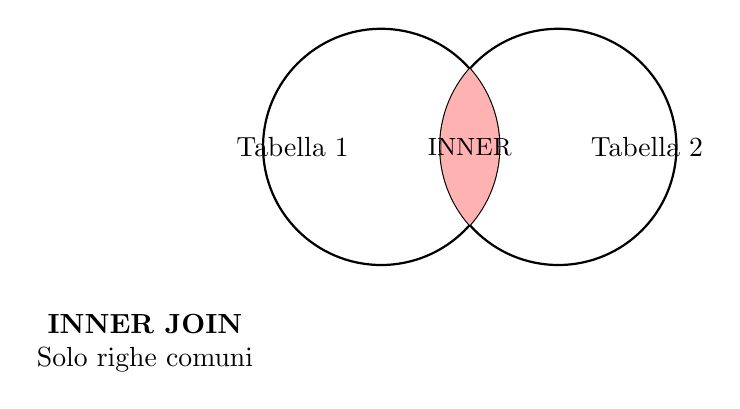
\begin{tikzpicture}[scale=1.5]
        % Cerchi
        \draw[thick] (0,0) circle (1);
        \draw[thick] (1.5,0) circle (1);

        % Etichette
        \node at (-0.75, 0) {Tabella 1};
        \node at (2.25, 0) {Tabella 2};

        % Area JOIN (intersezione)
        \begin{scope}
            \clip (0,0) circle (1);
            \fill[red!30] (1.5,0) circle (1);
        \end{scope}

        \node at (0.75, 0) {\small INNER};
        \node at (-2, -1.5) {\textbf{INNER JOIN}};
        \node at (-2, -1.8) {Solo righe comuni};
    \end{tikzpicture}
    \caption{INNER JOIN: intersezione}
\end{figure}

\subsection{Esempio}

\begin{lstlisting}[language=SQL, caption=INNER JOIN]
-- Trovare clienti e loro ordini
SELECT
    c.idCliente,
    c.nome,
    c.cognome,
    o.idOrdine,
    o.dataOrdine,
    o.totale
FROM cliente c
INNER JOIN ordine o ON c.idCliente = o.idCliente;
\end{lstlisting}

Risultato: Solo clienti che hanno fatto almeno un ordine.

\subsection{INNER JOIN su condizioni multiple}

\begin{lstlisting}[language=SQL, caption=INNER JOIN su più colonne]
-- Trovare ordini e i prodotti ordinati
SELECT
    o.idOrdine,
    p.nome AS nomeProdotto,
    op.quantita,
    op.prezzo_unitario
FROM ordine o
INNER JOIN ordine_prodotto op ON o.idOrdine = op.idOrdine
INNER JOIN prodotto p ON op.idProdotto = p.idProdotto;
\end{lstlisting}

\section{LEFT JOIN}

LEFT JOIN restituisce TUTTE le righe della tabella di sinistra e le righe corrispondenti della tabella di destra. Se non c'è corrispondenza, le colonne di destra sono NULL.

\subsection{Diagramma Venn}

\begin{figure}[h]
    \centering
    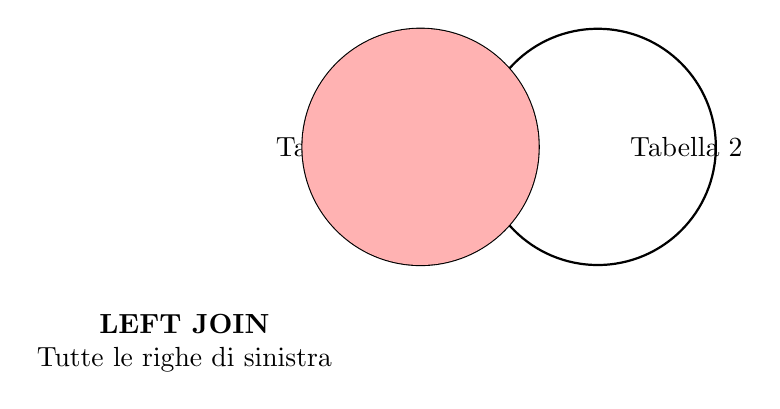
\begin{tikzpicture}[scale=1.5]
        % Cerchi
        \draw[thick] (0,0) circle (1);
        \draw[thick] (1.5,0) circle (1);

        % Etichette
        \node at (-0.75, 0) {Tabella 1};
        \node at (2.25, 0) {Tabella 2};

        % Area LEFT (tabella sinistra intera)
        \fill[red!30] (0,0) circle (1);

        \node at (-2, -1.5) {\textbf{LEFT JOIN}};
        \node at (-2, -1.8) {Tutte le righe di sinistra};
    \end{tikzpicture}
    \caption{LEFT JOIN: tutte le righe della tabella di sinistra}
\end{figure}

\subsection{Esempio}

\begin{lstlisting}[language=SQL, caption=LEFT JOIN]
-- Trovare TUTTI i clienti e i loro ordini
-- (inclusi clienti senza ordini)
SELECT
    c.idCliente,
    c.nome,
    c.cognome,
    COUNT(o.idOrdine) AS numOrdini,
    COALESCE(SUM(o.totale), 0) AS totalSpeso
FROM cliente c
LEFT JOIN ordine o ON c.idCliente = o.idCliente
GROUP BY c.idCliente, c.nome, c.cognome;
\end{lstlisting}

Risultato: Tutti i clienti, anche quelli senza ordini (che avranno numOrdini=0).

\subsection{Usare LEFT JOIN per trovare record ASSENTI}

\begin{lstlisting}[language=SQL, caption=LEFT JOIN per trovare mancanze]
-- Trovare clienti che NON hanno fatto ordini
SELECT
    c.idCliente,
    c.nome,
    c.cognome
FROM cliente c
LEFT JOIN ordine o ON c.idCliente = o.idCliente
WHERE o.idOrdine IS NULL;
\end{lstlisting}

Filtrando WHERE o.idOrdine IS NULL trovi esattamente i clienti senza ordini.

\section{RIGHT JOIN}

RIGHT JOIN è l'inverso di LEFT JOIN: restituisce tutte le righe della tabella di destra e le corrispondenze della sinistra.

\subsection{Esempio}

\begin{lstlisting}[language=SQL, caption=RIGHT JOIN]
-- Trovare TUTTI i prodotti e quante volte sono stati ordinati
SELECT
    p.idProdotto,
    p.nome,
    COUNT(op.idOrdine) AS volteOrdinato
FROM ordine_prodotto op
RIGHT JOIN prodotto p ON op.idProdotto = p.idProdotto
GROUP BY p.idProdotto, p.nome;
\end{lstlisting}

\begin{tcolorbox}[colback=orange!10, colframe=orange!60, title=Nota: LEFT vs RIGHT}
RIGHT JOIN può sempre essere convertito in LEFT JOIN invertendo l'ordine:

\begin{lstlisting}[language=SQL]
-- Equivalenti:
FROM ordine_prodotto op RIGHT JOIN prodotto p ...
FROM prodotto p LEFT JOIN ordine_prodotto op ...
\end{lstlisting}

Preferisci LEFT JOIN per coerenza (maggior leggibilità).
\end{tcolorbox}

\section{FULL OUTER JOIN}

FULL OUTER JOIN restituisce tutte le righe da ENTRAMBE le tabelle. Se non c'è corrispondenza, le colonne dell'altra tabella sono NULL.

\begin{tcolorbox}[colback=orange!10, colframe=orange!60, title=Nota: MySQL non supporta FULL OUTER JOIN}
MySQL non supporta nativamente FULL OUTER JOIN. Usa un'alternativa con UNION:

\begin{lstlisting}[language=SQL]
SELECT * FROM tabella1 LEFT JOIN tabella2 ...
UNION
SELECT * FROM tabella1 RIGHT JOIN tabella2 ...;
\end{lstlisting}
\end{tcolorbox}

\subsection{Simulare FULL OUTER JOIN in MySQL}

\begin{lstlisting}[language=SQL, caption=FULL OUTER JOIN simulato con UNION]
-- Trovare tutti i dati cliente e ordine
SELECT
    c.idCliente,
    c.nome,
    o.idOrdine,
    o.dataOrdine
FROM cliente c
LEFT JOIN ordine o ON c.idCliente = o.idCliente
UNION
SELECT
    c.idCliente,
    c.nome,
    o.idOrdine,
    o.dataOrdine
FROM cliente c
RIGHT JOIN ordine o ON c.idCliente = o.idCliente
WHERE c.idCliente IS NULL;
\end{lstlisting}

\section{CROSS JOIN}

CROSS JOIN produce il prodotto cartesiano: combina ogni riga della prima tabella con ogni riga della seconda (senza condizione ON).

\subsection{Sintassi}

\begin{lstlisting}[language=SQL, caption=CROSS JOIN]
SELECT *
FROM tabella1
CROSS JOIN tabella2;
\end{lstlisting}

\subsection{Esempio pratico}

\begin{lstlisting}[language=SQL, caption=CROSS JOIN pratico]
-- Generare tutte le combinazioni possibili di prodotti e colori
SELECT
    p.idProdotto,
    p.nome,
    c.colore
FROM prodotto p
CROSS JOIN colore c;

-- Risultato: ogni prodotto combinato con ogni colore
-- Se 100 prodotti e 5 colori, risultato = 500 righe
\end{lstlisting}

\begin{tcolorbox}[colback=red!10, colframe=red!60, title=Attenzione: CROSS JOIN può creare troppi dati!]
Un CROSS JOIN tra tabelle grandi produce MOLTISSIME righe. Usa con cautela!
\end{tcolorbox}

\section{JOIN su Più Tabelle}

Puoi combinare più di due tabelle con più JOIN.

\subsection{Sintassi}

\begin{lstlisting}[language=SQL, caption=JOIN multipli]
SELECT colonne
FROM tabella1
JOIN tabella2 ON ...
JOIN tabella3 ON ...
JOIN tabella4 ON ...
WHERE ...;
\end{lstlisting}

\subsection{Esempio: JOIN su 4 tabelle}

\begin{lstlisting}[language=SQL, caption=JOIN multipli pratico]
-- Trovare cliente, suoi ordini, prodotti ordinati e categorie
SELECT
    c.nome,
    o.dataOrdine,
    p.nome AS nomeProdotto,
    op.quantita,
    cat.nome AS categoria
FROM cliente c
INNER JOIN ordine o ON c.idCliente = o.idCliente
INNER JOIN ordine_prodotto op ON o.idOrdine = op.idOrdine
INNER JOIN prodotto p ON op.idProdotto = p.idProdotto
INNER JOIN categoria cat ON p.idCategoria = cat.idCategoria
WHERE c.idCliente = 5
ORDER BY o.dataOrdine DESC;
\end{lstlisting}

\section{Self-Join}

Un self-join è un join tra una tabella e se stessa. Utile per dati gerarchici o correlati.

\begin{lstlisting}[language=SQL, caption=Self-join]
-- Tabella: dipendente (idDipendente, nome, idDirigente)
-- Trovare ogni dipendente e il nome del suo dirigente

SELECT
    d.nome AS dipendente,
    m.nome AS dirigente
FROM dipendente d
LEFT JOIN dipendente m ON d.idDirigente = m.idDipendente;
\end{lstlisting}

Nota: Usi alias (d e m) per distinguere i due ruoli della stessa tabella.

\section{Alias per Tabelle}

Gli alias rendono le query più leggibili, specialmente con JOIN.

\begin{lstlisting}[language=SQL, caption=Alias per tabelle]
-- Con alias (consigliato)
SELECT
    c.idCliente,
    c.nome,
    COUNT(o.idOrdine) AS numOrdini
FROM cliente c
LEFT JOIN ordine o ON c.idCliente = o.idCliente
GROUP BY c.idCliente, c.nome;

-- Senza alias (lungo e meno leggibile)
SELECT
    cliente.idCliente,
    cliente.nome,
    COUNT(ordine.idOrdine) AS numOrdini
FROM cliente
LEFT JOIN ordine ON cliente.idCliente = ordine.idCliente
GROUP BY cliente.idCliente, cliente.nome;
\end{lstlisting}

\section{Errori Comuni in JOIN}

\subsection{Dimenticare la condizione ON}

\begin{tcolorbox}[colback=red!10, colframe=red!60, title=Errore: Mancante condizione ON]
\begin{lstlisting}[language=SQL]
-- Sbagliato: crea un CROSS JOIN involontario
SELECT * FROM cliente JOIN ordine;

-- Corretto
SELECT * FROM cliente JOIN ordine ON cliente.idCliente = ordine.idCliente;
\end{lstlisting}
\end{tcolorbox}

\subsection{Usare WHERE invece di ON}

\begin{lstlisting}[language=SQL, caption=ON vs WHERE]
-- LEFT JOIN con filtro errato
SELECT *
FROM cliente c
LEFT JOIN ordine o
WHERE c.idCliente = o.idCliente;  -- Sbagliato!
-- Questo filtra dopo il JOIN, trasformando LEFT in INNER

-- Corretto
SELECT *
FROM cliente c
LEFT JOIN ordine o ON c.idCliente = o.idCliente
WHERE o.totale > 100;  -- Filtra dopo JOIN
\end{lstlisting}

\section*{Riepilogo concetti chiave}

\begin{tcolorbox}[colback=gray!10, colframe=black!60, title=Concetti fondamentali]
\begin{itemize}
    \item \textbf{INNER JOIN}: solo righe comuni
    \item \textbf{LEFT JOIN}: tutte le righe di sinistra + corrispondenze
    \item \textbf{RIGHT JOIN}: tutte le righe di destra + corrispondenze
    \item \textbf{FULL OUTER JOIN}: tutte le righe da entrambe (usa UNION in MySQL)
    \item \textbf{CROSS JOIN}: prodotto cartesiano (usa con cautela)
    \item \textbf{Self-join}: tabella con se stessa (usa alias)
    \item Usa \textbf{ON} per la condizione, WHERE per filtri successivi
    \item \textbf{Alias} rendono query complesse più leggibili
\end{itemize}
\end{tcolorbox}

\section*{Esercizi}

\begin{enumerate}
    \item Scrivi un INNER JOIN per trovare ordini e i relativi clienti (nome, cognome) per ordini dell'anno 2023.

    \item Usa LEFT JOIN per trovare TUTTI i clienti e il numero di ordini effettuati. Includi clienti senza ordini (che avranno count=0).

    \item Usa LEFT JOIN con WHERE IS NULL per trovare clienti che NON hanno mai fatto ordini.

    \item Crea un query con 3 JOIN: cliente, ordine, ordine\_prodotto, prodotto. Mostra cliente, numero ordine e prodotto ordinato.

    \item Usa CROSS JOIN per generare tutte le combinazioni di città clienti e categorie prodotti (utilità: analisi di mercato per ogni territorio).

    \item Scrivi un self-join su una tabella dipendente per mostrare ogni dipendente con il nome del suo manager (dirigente).

    \item Analizza questa query e spiega perché LEFT JOIN diventa INNER JOIN:
    \begin{lstlisting}[language=SQL]
SELECT * FROM cliente c
LEFT JOIN ordine o ON c.idCliente = o.idCliente
WHERE o.dataOrdine > '2023-01-01';
    \end{lstlisting}
\end{enumerate}
